%% History:
% Pavel Tvrdik (26.12.2004)
%  + initial version for PhD Report
%
% Daniel Sykora (27.01.2005)
%
% Michal Valenta (3.12.2008)
% rada zmen ve formatovani (diky M. Duškovi, J. Holubovi a J. Žďárkovi)
% sjednoceni zdrojoveho kodu pro anglickou, ceskou, bakalarskou a diplomovou praci

% One-page layout: (proof-)reading on display
%%%% \documentclass[11pt,oneside,a4paper]{book}
% Two-page layout: final printing
\documentclass[11pt,twoside,a4paper]{book}
%=-=-=-=-=-=-=-=-=-=-=-=--=%
% The user of this template may find useful to have an alternative to these
% officially suggested packages:
\usepackage[czech, english]{babel}

\usepackage[T1]{fontenc} % pouzije EC fonty
% pripadne pisete-li cesky, pak lze zkusit take:
% \usepackage[OT1]{fontenc}
\usepackage[utf8]{inputenc}
%=-=-=-=-=-=-=-=-=-=-=-=--=%
% In case of problems with PDF fonts, one may try to uncomment this line:
%\usepackage{lmodern}
%=-=-=-=-=-=-=-=-=-=-=-=--=%
%=-=-=-=-=-=-=-=-=-=-=-=--=%
% Depending on your particular TeX distribution and version of conversion tools
% (dvips/dvipdf/ps2pdf), some (advanced | desperate) users may prefer to use
% different settings.
% Please uncomment the following style and use your CSLaTeX (cslatex/pdfcslatex)
% to process your work. Note however, this file is in UTF-8 and a conversion to
% your native encoding may be required. Some settings below depend on babel
% macros and should also be modified. See \selectlanguage \iflanguage.
%\usepackage{czech}  %%%%%\usepackage[T1]{czech} %%%%[IL2] [T1] [OT1]
%=-=-=-=-=-=-=-=-=-=-=-=--=%

%%%%%%%%%%%%%%%%%%%%%%%%%%%%%%%%%%%%%%%
% Styles required in your work follow %
%%%%%%%%%%%%%%%%%%%%%%%%%%%%%%%%%%%%%%%
\usepackage{graphicx}
%\usepackage{indentfirst} %1. odstavec jako v cestine.

% thesis formatting macros
\usepackage{k336_thesis_macros}

% work type
\newcommand\TypeOfWork{Diplomová práce} \typeout{Diplomova prace}

% study program
\newcommand\StudProgram{Otevřená informatika, Navazující magisterský}

% study branch
\newcommand\StudBranch{Softwarové inženýrství}

%
% Work title, author, etc.
%
\newcommand\WorkTitle{Validace principů objektového návrhu v kódu}
\newcommand\FirstandFamilyName{Bc. Martin Vejmelka}
\newcommand\Supervisor{Ing. Ondřej Macek}

% Pouzijete-li pdflatex, tak je prijemne, kdyz bude mit vase prace
% funkcni odkazy i v pdf formatu
\usepackage[
  pdftitle={\WorkTitle},
  pdfauthor={\FirstandFamilyName},
  bookmarks=true,
  colorlinks=true,
  breaklinks=true,
  urlcolor=red,
  citecolor=blue,
  linkcolor=blue,
  unicode=true,
]{hyperref}

% Extension posted by Petr Dlouhy in order for better sources reference (\cite{} command) especially in Czech.
% April 2010
% See comment over \thebibliography command for details.

\usepackage[square, numbers]{natbib}             % sazba pouzite literatury
%\usepackage{url}
%\DeclareUrlCommand\url{\def\UrlLeft{<}\def\UrlRight{>}\urlstyle{tt}}  %rm/sf/tt
%\renewcommand{\emph}[1]{\textsl{#1}}    % melo by byt kurziva nebo sklonene,
\let\oldUrl\url
\renewcommand\url[1]{<\texttt{\oldUrl{#1}}>}

\begin{document}

\selectlanguage{czech}

\iflanguage{czech}{
  \typeout{************************************************}
  \typeout{Zvoleny jazyk: cestina}
  \typeout{Typ prace: \TypeOfWork}
  \typeout{Studijni program: \StudProgram}
  \typeout{Obor: \StudBranch}
  \typeout{Jmeno: \FirstandFamilyName}
  \typeout{Nazev prace: \WorkTitle}
  \typeout{Vedouci prace: \Supervisor}
  \typeout{***************************************************}
  \newcommand\Department{Katedra počítačové grafiky a interakce}
  \newcommand\Faculty{Fakulta elektrotechnická}
  \newcommand\University{České vysoké učení technické v Praze}
  \newcommand\labelSupervisor{Vedoucí práce}
  \newcommand\labelStudProgram{Studijní program}
  \newcommand\labelStudBranch{Obor}
}{
  \typeout{************************************************}
  \typeout{Language: english}
  \typeout{Type of Work: \TypeOfWork}
  \typeout{Study Program: \StudProgram}
  \typeout{Study Branch: \StudBranch}
  \typeout{Author: \FirstandFamilyName}
  \typeout{Title: \WorkTitle}
  \typeout{Supervisor: \Supervisor}
  \typeout{***************************************************}
  \newcommand\Department{Department of Computer Science and Engineering}
  \newcommand\Faculty{Faculty of Electrical Engineering}
  \newcommand\University{Czech Technical University in Prague}
  \newcommand\labelSupervisor{Supervisor}
  \newcommand\labelStudProgram{Study Programme}
  \newcommand\labelStudBranch{Field of Study}
}

%
% Title page
%
\coverpagestarts

%
% Acknowledgements
%
\acknowledgements
\noindent
TODO: Zde můžete napsat své poděkování, pokud chcete a máte komu děkovat.

%
% Declaration
%
% TODO: supply valid date
\declaration{V~Praze dne 15.\,5.\,2008}

%
% Abstract
%
\abstractpage

TODO: Translation of Czech abstract into English.

% Prace v cestine musi krome abstraktu v anglictine obsahovat i
% abstrakt v cestine.
\vglue60mm

\noindent{\Huge \textbf{Abstrakt}}
\vskip 2.75\baselineskip

\noindent
TODO: Abstrakt práce by měl velmi stručně vystihovat její podstatu. Tedy čím se práce zabývá a co je jejím výsledkem/přínosem.

\noindent
Očekávají se cca 1 -- 2 odstavce, maximálně půl stránky.

%
% Table of Contents
%
\tableofcontents

%
% List of Figures
%
\listoffigures

%
% List of Tables
%
\listoftables


%**************************************************************

\mainbodystarts
% horizontalní mezera mezi dvema odstavci
%\parskip=5pt
%11.12.2008 parskip + tolerance
\normalfont
\parskip=0.2\baselineskip plus 0.2\baselineskip minus 0.1\baselineskip

% Odsazeni prvniho radku odstavce resi class book (neaplikuje se na prvni
% odstavce kapitol, sekci, podsekci atd.) Viz usepackage{indentfirst}.
% Chcete-li selektivne zamezit odsazeni 1. radku nektereho odstavce,
% pouzijte prikaz \noindent.

%**************************************************************

% Pro snadnejsi praci s vetsimi texty je rozumne tyto rozdelit
% do samostatnych souboru nejlepe dle kapitol a tyto potom vkladat
% pomoci prikazu \include{jmeno_souboru.tex} nebo \include{jmeno_souboru}.
% Napr.:
% \include{1_uvod}
% \include{2_teorie}
% atd...

%*****************************************************************************
\chapter{Úvod}
Úvod charakterizující kontext zadání, případně motivace.

Výsledná struktura vaší práce a názvy a rozsahy jednotlivých kapitol se samozřejmě budou lišit podle typu práce a podle konkrétní povahy zpracovávaného tématu. Níže uvedená struktura práce odpovídá \textit{práci implementační}, viz \cite{infodp} respektive \cite{infobp}.


%*****************************************************************************
\chapter{Popis problému, specifikace cíle}

\begin{itemize}
\item Popis řešeného problému, vymezení cílů DP/BP a požadavků na implementovaný systém.
\item Popis struktury DP/BP ve vztahu k vytyčeným cílům.
\item Rešeršní zpracování existujících implementací, pokud jsou známy.
\end{itemize}

%*****************************************************************************
\chapter{Analýza a návrh řešení}
Analýza a návrh implementace (včetně diskuse různých alternativ a volby implementačního prostředí).


%*****************************************************************************
\chapter{Realizace}
Popis implementace/realizace se zaměřením na nestandardní části řešení.


%*****************************************************************************
\chapter{Testování}

\begin{itemize}
 \item Způsob, průběh a výsledky testování.
 \item Srovnání s existujícími řešeními, pokud jsou známy.
\end{itemize}


%*****************************************************************************
\chapter{Závěr}

\begin{itemize}
\item Zhodnocení splnění cílů DP/BP a  vlastního přínosu práce (při formulaci je třeba vzít v potaz zadání práce).
\item Diskuse dalšího možného pokračování práce.
\end{itemize}

%*****************************************************************************
% Seznam literatury je v samostatnem souboru reference.bib. Ten
% upravte dle vlastnich potreb, potom zpracujte (a do textu
% zapracujte) pomoci prikazu bibtex a nasledne pdflatex (nebo
% latex). Druhy z nich alespon 2x, aby se poresily odkazy.

% originally following specification for bibliography formating was used
%\bibliographystyle{abbrv}

% Here is an improvment by Petr Dlouhy (April 2010).
% It is mainly for supervisors who expect Czech fomrating rules for references
% Additional feature is live url addresses to sources from your pdf file
% It requires the file csplainnat.bst (included in this sample zipfile).

\bibliographystyle{csplainnat}

%bibliographystyle{plain}
%\bibliographystyle{psc}
{
%JZ: 11.12.2008 Kdo chce mit v techto ukazkovych odkazech take odkaz na CSTeX:
\def\CS{$\cal C\kern-0.1667em\lower.5ex\hbox{$\cal S$}\kern-0.075em $}
\bibliography{reference}
}

% M. Dušek radi:
%\bibliographystyle{alpha}
% kdy citace ma tvar [AutorRok] (napriklad [Cook97]). Sice to asi neni  podle ceske normy (BTW BibTeX stejne neodpovida ceske norme), ale je to nejprehlednejsi.
% 3.5.2009 JZ polemizuje: BibTeX neobvinujte, napiste a poskytnete nam styl (.bst) splnujici citacni normu CSN/ISO.

%*****************************************************************************
%*****************************************************************************
\appendix

% JZ: 3.5.2009 \chapter z book zajistí automaticky
%\subsection{Začátky kapitol na liché stránky}
%Ve výsledném textu je dobré, když každá kapitola začíná na liché stránce. Tedy použijte:
%\begin{verbatim}
%  \cleardoublepage\include{1_uvod}
%  \cleardoublepage\include{2_teorie}
%   atd.\ldots{}
%\end{verbatim}

%
% Abbreviation list
%
\chapter{Seznam použitých zkratek}

\begin{description}
\item[2D] Two-Dimensional
\item[ABN] Abstract Boolean Networks
\item[ASIC] Application-Specific Integrated Circuit
\end{description}
\vdots

%*****************************************************************************
\chapter{UML diagramy}
\textbf{\large Tato příloha není povinná a zřejmě se neobjeví v každé práci. Máte-li ale větší množství podobných diagramů popisujících systém, není nutné všechny umísťovat do hlavního textu, zvláště pokud by to snižovalo jeho čitelnost.}

%*****************************************************************************
\chapter{Instalační a uživatelská příručka}
\textbf{\large Tato příloha velmi žádoucí zejména u softwarových implementačních prací.}

%*****************************************************************************
\chapter{Obsah přiloženého CD}
\textbf{\large Tato příloha je povinná pro každou práci. Každá práce musí totiž obsahovat přiložené CD. Viz dále.}

Může vypadat například takto. Váš seznam samozřejmě bude odpovídat typu vaší práce. (viz \cite{infodp}):

\begin{figure}[h]
\begin{center}
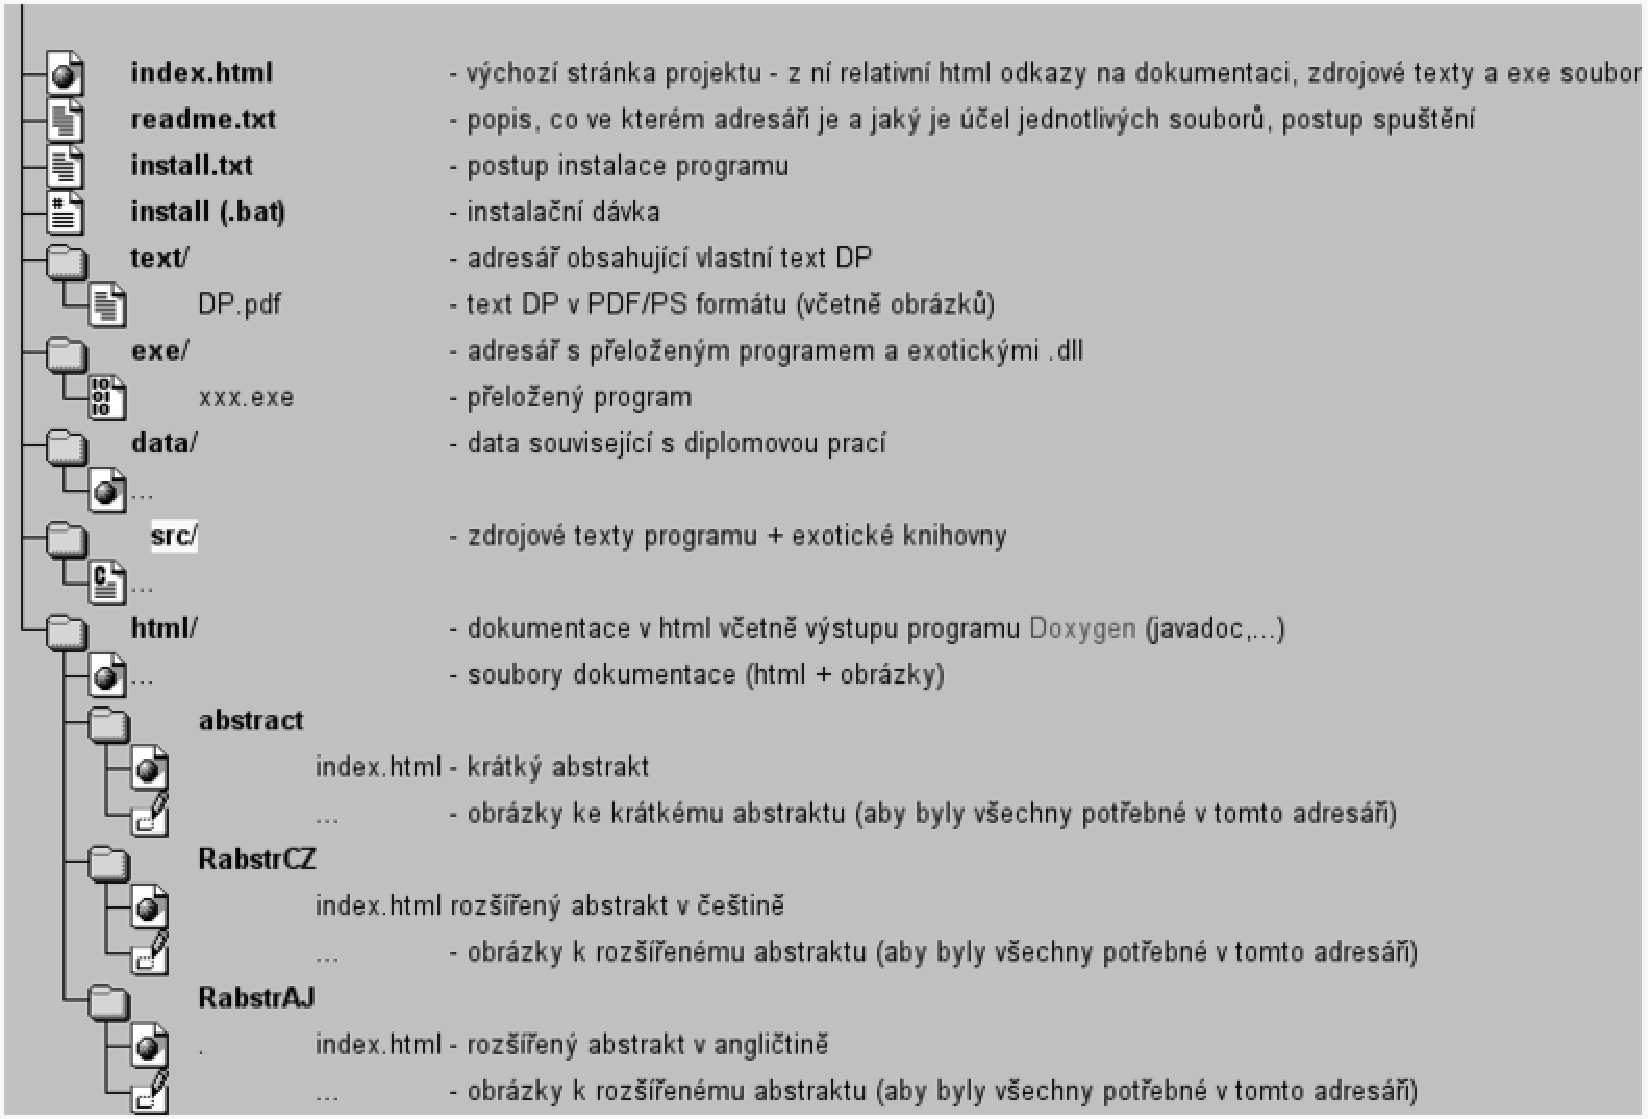
\includegraphics[width=14cm]{figures/seznamcd}
\caption{Seznam přiloženého CD --- příklad}
\label{fig:seznamcd}
\end{center}
\end{figure}

Na GNU/Linuxu si strukturu přiloženého CD můžete snadno vyrobit příkazem:\\
\verb|$ tree . >tree.txt|\\
Ve vzniklém souboru pak stačí pouze doplnit komentáře.

Z \textbf{README.TXT} (případne index.html apod.)  musí být rovněž zřejmé, jak programy instalovat, spouštět a jaké požadavky mají tyto programy na hardware.

Adresář \textbf{text}  musí obsahovat soubor s vlastním textem práce v PDF nebo PS formátu, který bude později použit pro prezentaci diplomové práce na WWW.

\end{document}
